\section{Boilerplate Detection and Removal}\label{sec:boilerplate_removal}

A web page is a document that contains both content and presentation information.
The content of a web page is the information that is relevant to the user, while the presentation information is the information that is used to display the web page.
Boilerplate refers to the presentation information that is not relevant to the user, such as navigation menus, advertisements, and other non-content elements.

\begin{figure}[h]
    \centering
    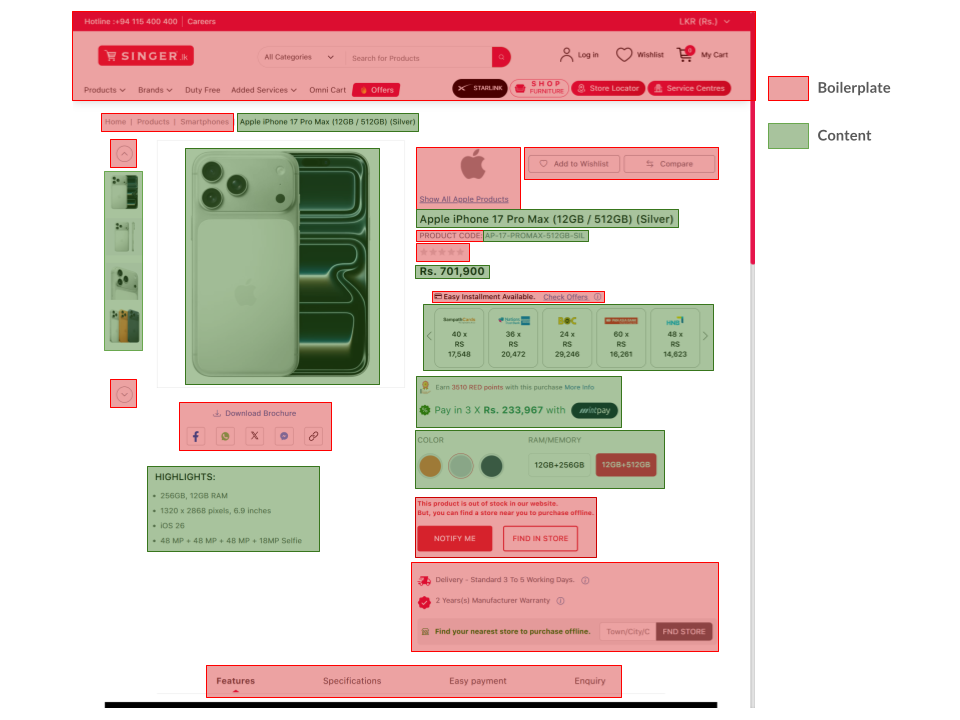
\includegraphics[width=0.8\textwidth]{images/boilerplate_vs_content}~\caption{Boilerplate vs. content on a web page}
    \label{fig:boilerplate_vs_content}
\end{figure}

Boilerplate detection and removal is the process of identifying and removing boilerplate from a web page so that only the relevant content remains.
This is an important task for many applications, such as web scraping, information retrieval, and natural language processing as boilerplate/template content can interfere with the accuracy of these applications.

There are primarily two approaches to boilerplate detection and removal\cite{pomikalek2011removing}:
\begin{enumerate}
    \item \textbf{Site-Level Methods}: These methods analyze multiple pages from the same website to identify common patterns and structures that are likely to be boilerplate.
    By comparing the structure and content of different pages, site-level methods can effectively identify and remove boilerplate elements that are consistent across the site.

    \item \textbf{Page-Level Methods}: These methods analyze each page individually to identify boilerplate elements based on features such as link density, text density, and the structure of the HTML document.
\end{enumerate}

\subsection{Site-Level Methods}\label{subsec:site-level-methods}

\subsubsection{Site Style Trees (SST)}\label{subsubsec:site-style-trees}
Using the DOM from a sample of pages from a website, a site style tree (SST) can be constructed to represent the common structure of that specific website.
For each unique subtree which appears in the SST, a count is maintained to track how many pages contain that subtree.
Subtrees that appear in a large number of pages are likely to be boilerplate, while those that appear in fewer pages are more likely to be content.
By analyzing the SST, it is possible to identify and remove boilerplate elements from the pages of the website, leaving only the relevant content. \cite{yi2003eliminating}

\begin{figure}[h]
    \centering
    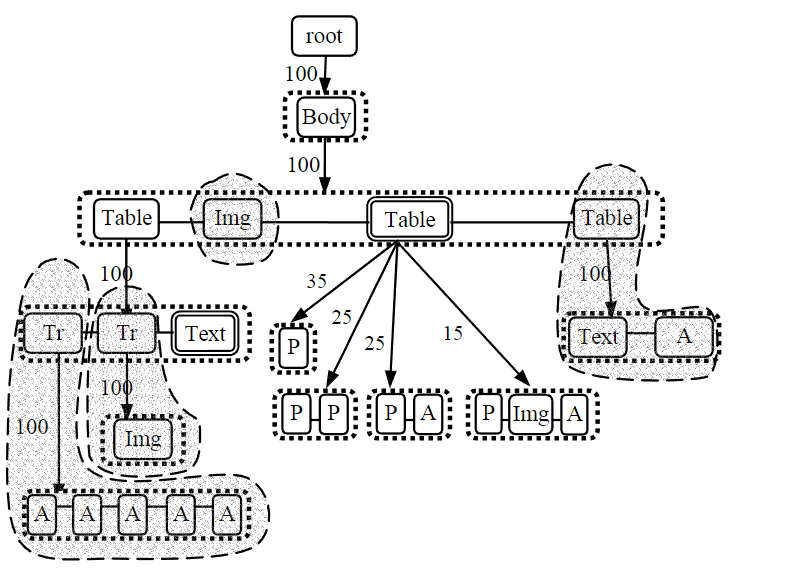
\includegraphics[width=0.8\textwidth]{images/site_style_trees_example}~\caption{An example of site style trees (SST)\cite{yi2003eliminating}}
    \label{fig:site_style_trees_example}
\end{figure}

\subsubsection{Using Subtree Hashes}\label{subsubsec:subtree-hashes}
Similar to site style trees, subtree hashes can be used to identify boilerplate elements across multiple pages of a website.
By computing a hash for each subtree in the DOM of a page, it is possible to compare these hashes across different pages to identify common subtrees that are likely to be boilerplate.
Subtrees that have the same hash across multiple pages are likely to be boilerplate, while those that have unique hashes are more likely to be content.
This method can be computationally efficient and effective in identifying boilerplate elements. \cite{gibson2005volume}

\subsection{Page-Level Methods}\label{subsec:page-level-methods}

\subsubsection{Body Text Extraction (BTE)}\label{subsubsec:body-text-extraction}
This is a heuristic-based method based on the observation that the main content of a web page usually contains long streams of uninterrupted text with a low HTML tag density.
By analyzing the structure of the HTML document and identifying areas with high text density and low tag density, it is possible to extract the main content of the page.
While this is a simple method, one major drawback is that modern web pages are extremely complex and may not always follow this pattern, leading to inaccurate results. \cite{vogels2018web2text}

\subsubsection{Shallow Text Features}\label{subsubsec:shallow-text-features}
This method first chunks the web page into smaller sections based on the structure of the HTML document.
It then computes various features for each chunk, such as link density (the ratio of links to text), text density (the ratio of text to HTML tags), and other structural features.
High link density is generally indicative of boilerplate, while high text density is more indicative of content. \cite{kohlschutter2010boilerplate}

This also builds on the concept of functional short text vs descriptive long text, where functional short text,
characterized by short, incomplete sentences  (e.g., home, contact us) is more likely to be boilerplate,
while descriptive long text, characterized by full sentences and higher complexity is more likely to be content. \cite{kohlschutter2010boilerplate}

\subsubsection{Supervised Machine Learning Techniques}\label{subsubsec:supervised-ml-methods}
While BTE and shallow text features can be effective in some cases, they may not always be sufficient to accurately identify boilerplate elements, especially on modern web pages with complex structures.
Supervised machine learning techniques, such as neural networks and multi-layer perceptrons (MLPs), can be trained on labeled datasets of web pages to learn more complex patterns and features that distinguish boilerplate from content.
By using a large and diverse training dataset, these models can learn to generalize well to new web pages and can be more effective in accurately identifying boilerplate elements.
These techniques generally show a significant improvement in performance compared to heuristic-based methods, especially on modern web pages with complex structures. \cite{schafer2017accurate}

Two examples of supervised machine learning techniques for boilerplate detection and removal are Web2Text\cite{vogels2018web2text},
which uses Convolutional Neural Networks (CNNs) to predict probabilities for chunks of a page, and the transition between blocks,
and BoilerNet\cite{leonhardt2020boilerplate}, which use bidirectional LSTMs that learn dependency between blocks and their neighbours.

\subsection{Performance Improvements}\label{subsec:performance-improvements}
Removing boilerplate content from web pages have shown to significant performance gains in downstream tasks such as
web page classification and clustering, as it allows these tasks to focus on the relevant content of the page rather than being distracted by irrelevant boilerplate elements.
In addition, it also reduces the amount of data that needs to be processed, which can lead to faster processing times and improved efficiency in these tasks.

Using site style trees (SSTs) to remove boilerplate has been shown to improve the accuracy in web page classification tasks from
0.625 to 0.954\cite{yi2003eliminating}.
Using the same method, the average F1-score for k-means clustering also improved from 0.506 to 0.751.

\subsection{Summary}\label{subsec:boilerplate_summary}

Boilerplate detection and removal is a problem with a number of possible approaches ranging from simple rule-based models to deep learning models.
Site-level methods are effective when multiple pages from the same website are available, while page-level methods operate on individual pages without any prior site knowledge.
Supervised machine learning techniques offer the highest accuracy but require labeled training data.
Table~\ref{tab:boilerplate_summary} summarises the key approaches reviewed in this section.

\begin{table}[h]
    \centering
    \small
    \renewcommand{\arraystretch}{1.4}
    \begin{tabularx}{\textwidth}{p{4cm} p{2.2cm} X X}
        \toprule
        \textbf{Method} & \textbf{Type} & \textbf{Strengths} & \textbf{Limitations} \\
        \midrule
        Site Style Trees (SST)\cite{yi2003eliminating} & Site-level & Cross-page detection, improves classification \& clustering & Needs multiple pages from same site \\
        Subtree hashes\cite{gibson2005volume} & Site-level & Efficient, easy to implement & Needs multiple pages, fragile to DOM changes \\
        Body Text Extraction (BTE)\cite{vogels2018web2text} & Page-level & No training data, lightweight & Poor accuracy on complex pages \\
        Shallow text features\cite{kohlschutter2010boilerplate} & Page-level & Interpretable, no training data & Hand-crafted heuristics, limited generalisation \\
        Web2Text\cite{vogels2018web2text} & Page-level & Learns complex patterns & Requires labeled data \\
        BoilerNet\cite{leonhardt2020boilerplate} & Page-level & Models block dependencies, best accuracy & Requires labeled data, higher complexity \\
        \bottomrule
    \end{tabularx}
    \caption{Summary of boilerplate detection and removal approaches}
    \label{tab:boilerplate_summary}
\end{table}
